\section{Introduction}
\begin{figure*}[t]
\centering
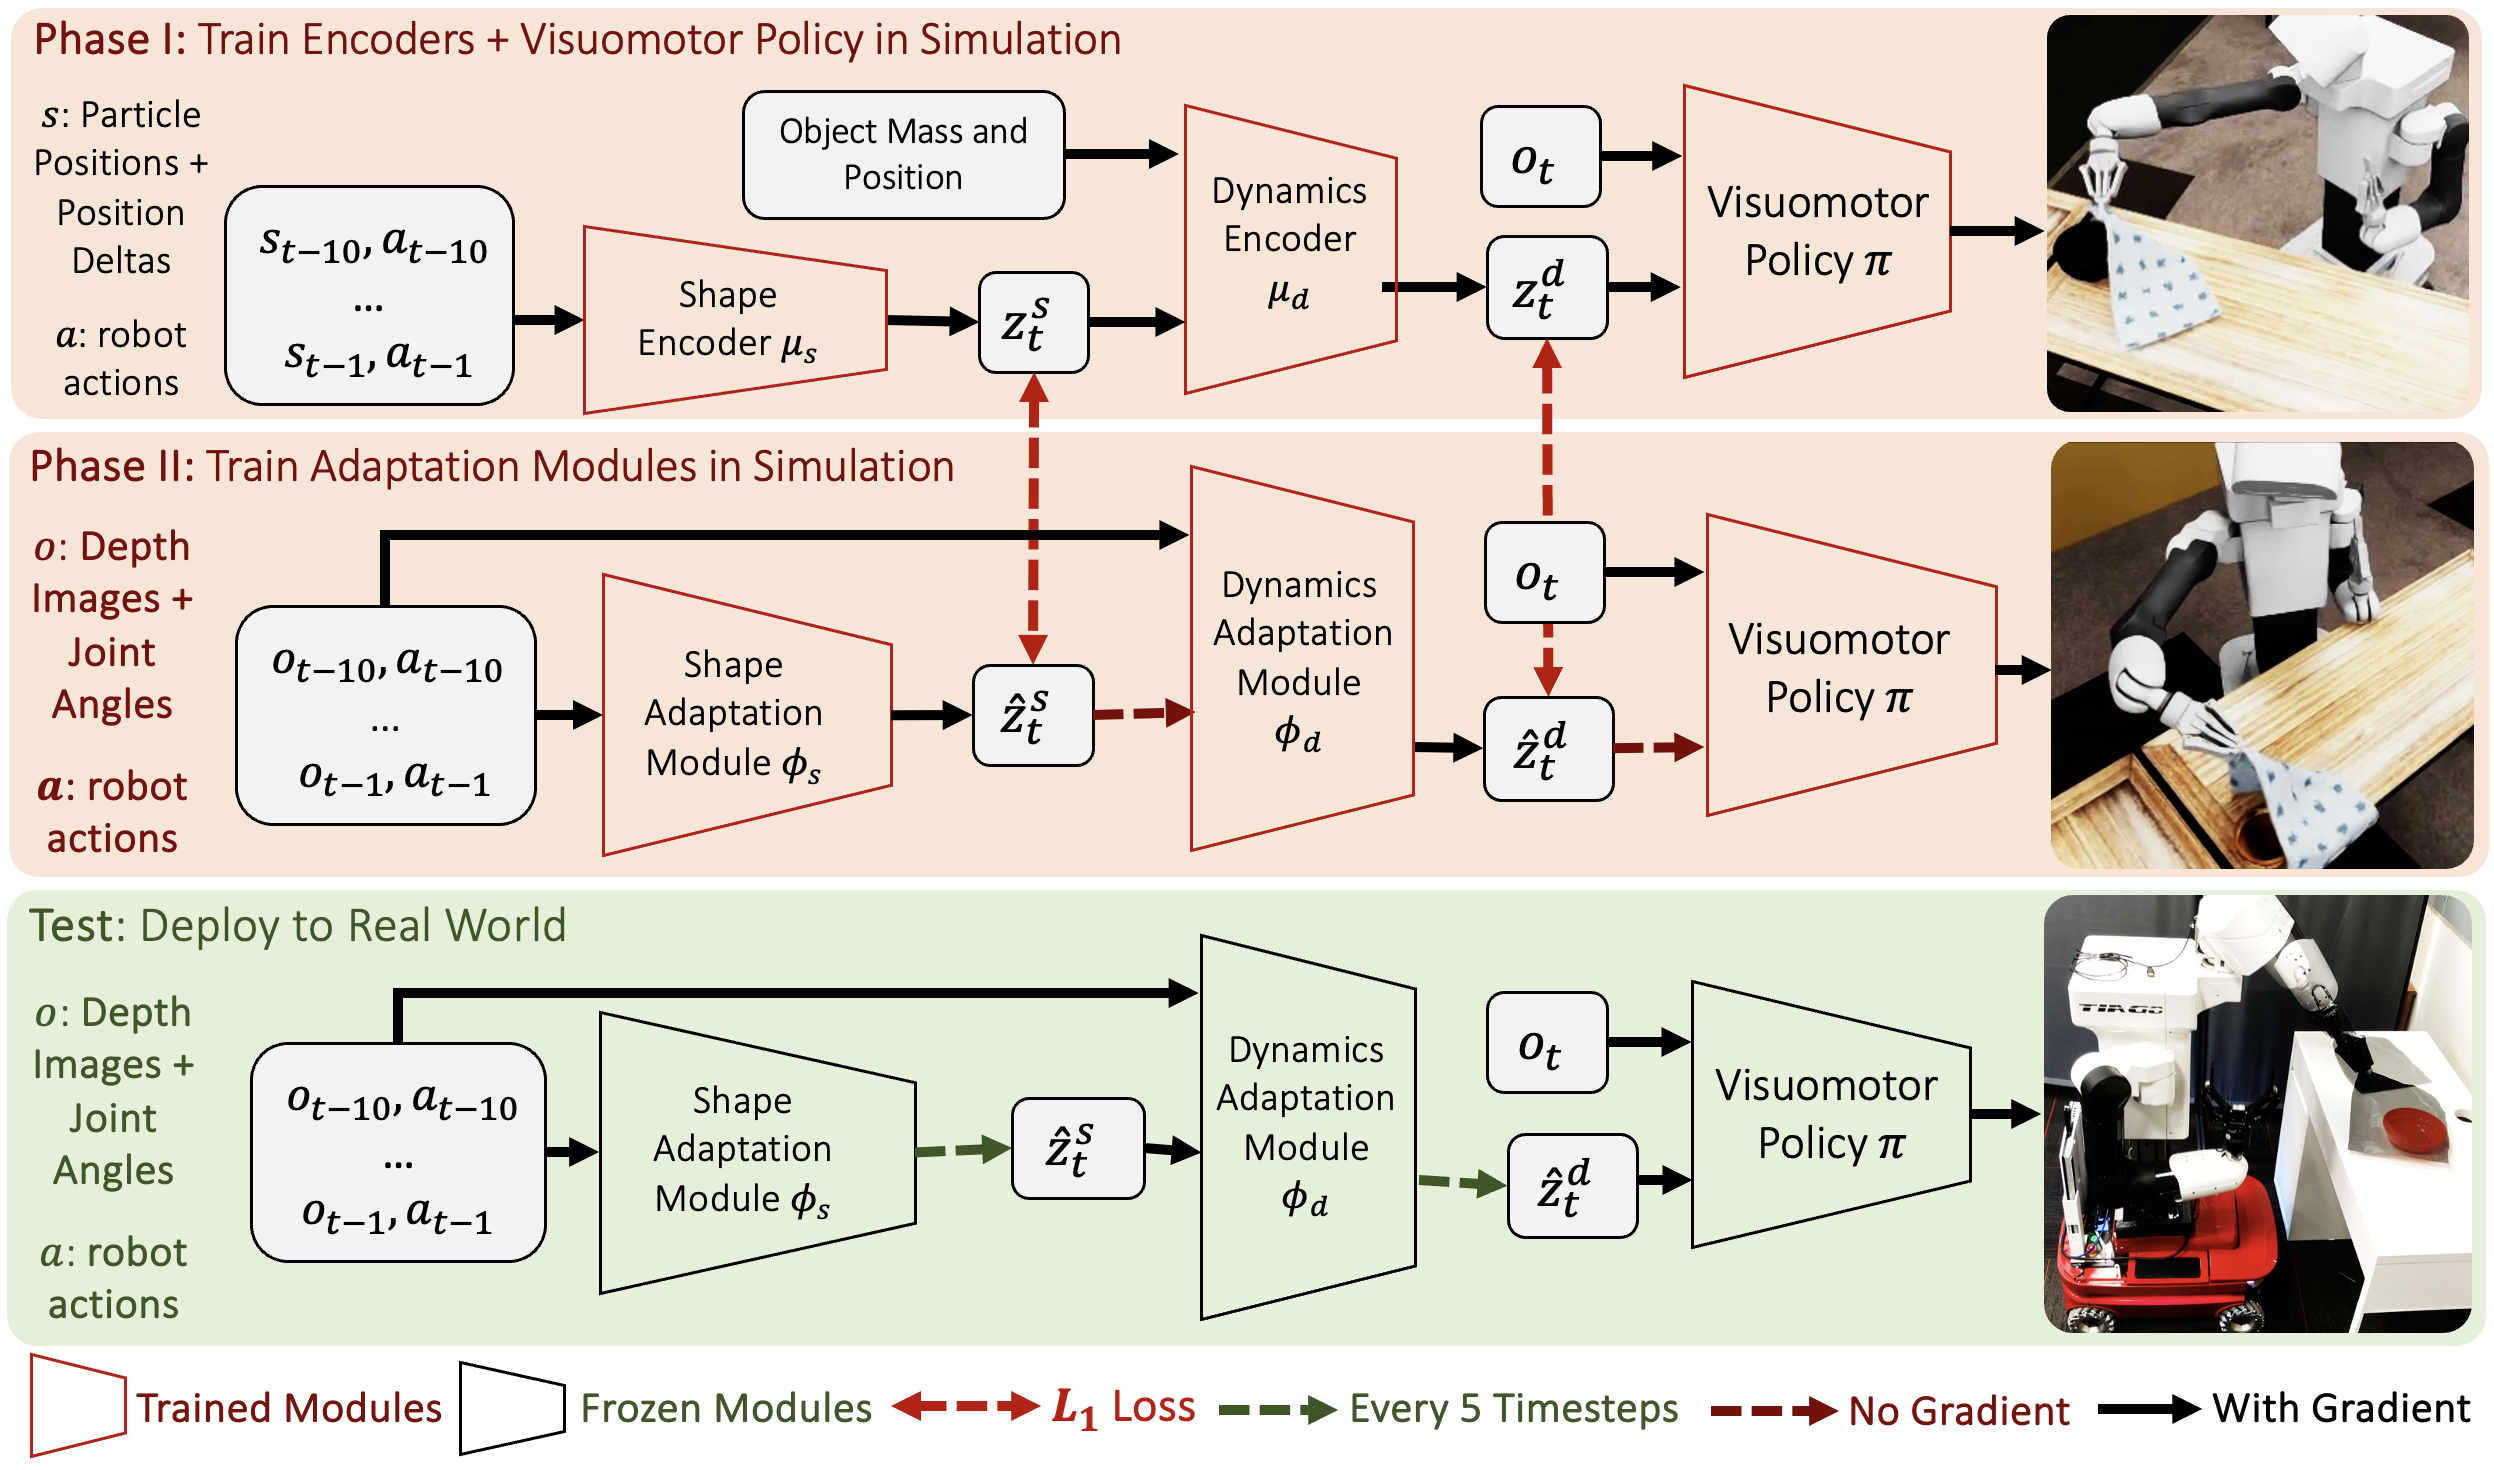
\includegraphics[width=\textwidth]{photos/rda.png}
\caption{\small \textbf{The \methodname{} Method}. 
Below we explain training (\textit{\textcolor{Orange}{top and middle}}) in simulation and deploying in the real world (\textit{\textcolor{OliveGreen}{bottom}}) a deformable object mobile manipulation solution with \methodname{}.
Training with \methodname{} (\textit{\textcolor{Orange}{top and middle}}) is a two-step procedure. In the first step (\textit{\textcolor{Orange}{top}}), the agent is asked to solve a simulated version of the task by learning a visuomotor policy and two encoders: a Shape Encoder, $\mu_{s}$, and a Dynamics Encoder, $\mu_{d}$, using privileged state information of the object from the simulator, such as mass and particle positions. In the second step (\textit{\textcolor{Orange}{middle}}), \methodname{} frees itself from privileged simulator information by learning a new Shape Adaptation module, $\phi_{s}$, and Dynamics Adaptation module $\phi_{d}$, using L1-losses to replace the Shape Encoder and the Dynamics Encoder, respectively. At test time (\textit{\textcolor{OliveGreen}{bottom}}), both the Shape and Dynamics adaptation modules and the visuomotor policy are directly deployed to the real world, with the adaptation modules updating the Shape Embedding $\hat{z}_t^{s}$ and Dynamics Embeddings $\hat{z}_t^{d}$ to the visuomotor policy once every 5 timesteps.}
\vspace{-10pt}
\label{fig:rda}
\end{figure*}
\label{s_intro}

Deformable objects, such as cables and clothes, can change in shape. As a result, the optimal strategies for deformable object manipulation often rely heavily on the object's dynamics, such as material properties, which are unknown a priori. For example, consider covering the top of a bowl with a 2D deformable object, such as a hat or a piece of cloth. For a hat, thanks to its high rigidity, a simple pick-and-place motion would be sufficient. But for a cloth, because of its softness, a fling followed by a sweep-and-cover motion is necessary. However, the dynamics of deformable objects are not fully observable a priori, and we as humans adapt to their dynamics in real-time \textit{during} our interaction with them. As we grasp and lift a hat or a cloth, we swiftly infer its material properties and adjust our placing motion or flinging speed to cover the bowl entirely. This rapid adaptation of unknown dynamics enables humans to efficiently manipulate deformable objects across diverse dynamics, categories, and instances, and we hope to endow robots with similar capabilities.

While many existing solutions can perform various deformable object manipulation tasks, generalizing these solutions to in-the-wild settings across diverse deformable object dynamics, categories, and instances remains challenging. For example, state estimation methods model deformable objects using state representations such as particles~\cite{jaillet1998deformable,li2018learning}, edges~\cite{triantafyllou2016geometric,yuba2017unfolding}, and graphs~\cite{longhini2023edo,lippi2020latent}, but they require full object observability and therefore cannot handle object occlusions. In parallel, a system identification method such as~\cite{chebotar2019closing} tries to estimate the deformable object's physics parameters from real-robot trajectories and then fine-tune the manipulation strategy in simulation, but this method requires multiple trajectories and therefore cannot adapt to unknown dynamics in real-time. Prior methods have also attempted to learn generalizable deformable object manipulation from large-scale cross-embodiment robotics datasets~\cite{black2024pi0,kim2024openvla}, but due to their limited scale, zero-shot generalization to a new robot embodiment remains challenging. Finally, other methods have also applied Rapid Motor Adaptation~\cite{kumar2021rma} to other robotics tasks such as legged locomotion~\cite{kumar2022adapting}, in-hand manipulation~\cite{qi2023hand}, and simulated robotic manipulation~\cite{liang2024rapid}. However, applying RMA to deformable object mobile manipulation presents an added complexity: the dynamics of the deformable object includes not only its mass and position, but also how the shape of the object changes. 

\begin{figure*}[t]
\centering
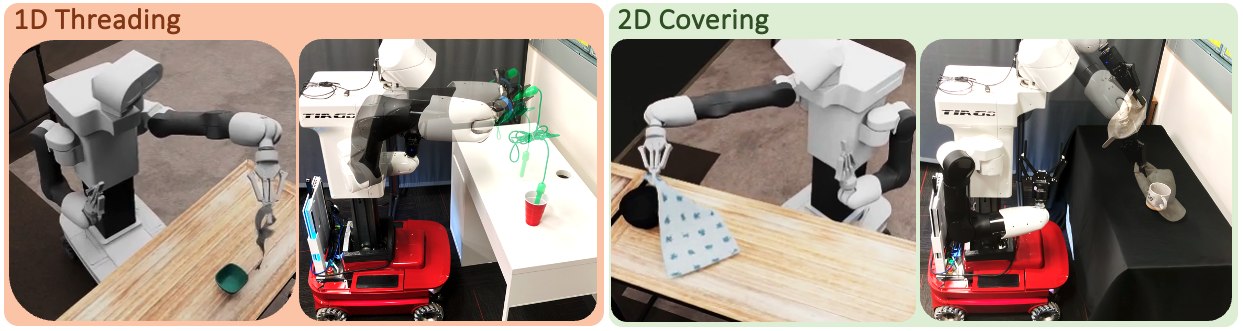
\includegraphics[trim=0cm 0cm 0cm 0cm, clip, width=\linewidth]{photos/real.png}
\caption{\textbf{Simulated and Real-World Version of the Two Tasks}: \taskone~(\textcolor{Orange}{\textit{Left Half}}) and \tasktwo~(\textcolor{OliveGreen}{\textit{Right Half}}). Each task is trained in simulation (\textit{left image of each half}) and then deployed directly to the real world (\textit{right image of each half}) under unseen objects, environments, and lighting conditions. By interacting with deformable objects across a broad range of instances, geometries, and categories in simulation, \methodname{} successfully learns a visuomotor policy that adapts to and excels at manipulating real-world deformable objects of unseen dynamics, instances, and categories on a real bimanual mobile manipulator.}
\label{fig:tasks}
\vspace{-15px}
\end{figure*}
In this work, our key insight is that the recent ground-truth particle positions of a deformable object in simulation capture changes in the object's shape, making it possible to extend the RMA framework to learn to manipulate deformable objects with unknown dynamics.
This key insight allows us to create a novel two-phase method for learning to manipulate real-world deformable objects by inferring and adapting to their unknown dynamics: First, in a simulated version of the task, we train a visuomotor policy that is conditioned on a dynamics embedding of privileged simulator information, such as the recent ground-truth particle positions as well as the mass and position of the deformable object. 
Second, we learn a dynamics adaptation module in simulation to predict the dynamics embedding learned in the first step, using only non-privileged information, such as the robot's recent visual observations and actions. 
At test time, since the dynamics adaptation module and the visuomotor policy are learned in simulation using only onboard visual sensor signals, we can directly transfer them to a real robot to accomplish a deformable object mobile manipulation task. 
We call this method \textbf{\methodname{}} from \textbf{\underline{R}}apid \textbf{\underline{A}}daptation of \textbf{\underline{P}}art\underline{i}cle \textbf{\underline{D}}ynamics (Fig.~\ref{fig:pull}).

We evaluated \methodname{} in two real-robot deformable object mobile manipulation tasks involving 1D and 2D deformable objects with unseen dynamics, categories, and instances: \taskone~and \tasktwo. \methodname{} significantly outperforms existing state-of-the-art methods by 65\%+ success rates in both tasks based only on onboard visual inputs. This indicates that \methodname{}'s online adaptation algorithm provides a general and versatile mechanism for learning to manipulate deformable objects with unknown dynamics in simulation and then transferring the learned policies to the real world across a wide range of unseen deformable object dynamics, categories, and instances.